\documentclass[UTF8,11pt,a4paper]{ctexart}
\usepackage[margin=2.2cm]{geometry}
\usepackage{amsmath,amssymb,booktabs,graphicx,microtype,natbib}
\usepackage[colorlinks=true,allcolors=blue]{hyperref}
\usepackage{caption}
\captionsetup{font=small,labelfont=bf}
\graphicspath{{figures/}}
\setlength{\parindent}{2em}
\setlength{\parskip}{0.25em}

\title{从经验除霜成本到视觉决策状态：\\空气源热泵原始运行数据的可审计离线框架}
\author{作者信息待补充}
\date{论文初稿演示版，\today}

\begin{document}
\maketitle

\begin{abstract}
空气源热泵的除霜启动是一个序贯决策：延迟除霜可避免供热中断，但结霜会逐步增加电耗与供热服务缺口；过早除霜则支付不必要的除霜和恢复代价。历史数据只记录控制器实际采取的一次动作，因而既缺少反事实结果，也缺少可直接赋给结霜图像的决策标签。本文提出一条从约1秒原始水侧与电功率数据到图像监督信号的可审计链路。我们首先从50个有效除霜--恢复事件估计经验除霜“门票”，并在固定观察策略下构造逐循环更新成本曲线。在77个目录循环中，47个具有完整观察候选域，另有12个可作为传感器终点右截尾敏感性分析；完整循环中37个得到内部最小值，10个最小值位于右边界。经验最优点相对实际除霜提前量的中位数为58.8分钟，但1\%低遗憾区宽度中位数为33.0分钟，表明单一时刻标签通常过于尖锐。基于逐图遗憾标签的11实验留一评估显示，冻结40维RGB特征的最佳组合为前视机位与RBF支持向量机，平衡准确率为0.965（95\%实验bootstrap区间0.942--0.987）；五类模型之间的差异小于机位差异。然而，对15个本地可用循环、3个实验的开发性分析未支持“最优时刻对应的单帧视觉状态更集中”：全机位最优邻域相对固定时间的质心离散度差为$+0.064$（0.033--0.081，负值才支持该命题）。因此，本框架完成了从成本到图像标签的方法链路，同时把下一步需求收敛为前瞻干预与RGB--传感器历史融合，而不是继续无约束地增加图像模型复杂度。本文结果均为固定经验门票下的离线策略条件估计，不代表因果全局最优、已实现节能或直接热舒适改善。
\end{abstract}

\section{引言}
室外换热器结霜会限制空气流动与传热，而除霜过程又会中断有效供热并消耗电能。因此，控制器需要在继续结霜运行的损失与立即除霜的固定代价之间作出权衡。既有研究已从名义供热损失、霜量跟踪和模型控制角度研究最优除霜启动\citep{wang2020,li2020,chung2021,klingebiel2025}；图像识别也已用于按需除霜与供热性能评估\citep{chen2022,wang2024}. 真正未解决的环节不是“能否看见霜”，而是如何把只有一次实际动作的历史循环转换为每张图像可学习、同时保留决策不确定性的监督信号。

直接把成本函数的数学最小点当作唯一标签会产生两个问题。第一，多个候选时刻可能具有近似相同成本；在最小点两侧强行赋予相反类别，会把近似等价的视觉状态变成标签噪声。第二，相邻图像和同实验循环高度相关，随机按帧划分会泄露机位、曝光与实验条件\citep{roberts2021}. 因此，可靠链路必须同时输出逐时刻成本遗憾、按循环或实验隔离的评估，以及能检验模型是否只学习时间进程的对照。

本文的核心论证是：原始运行数据可以在明确的经验策略假设下形成可追溯的成本曲线；相对遗憾比单一最小点更适合定义视觉标签；但高分类准确率并不自动证明最优视觉状态跨循环集中。我们依次审计候选域、比较九个机位组与五种模型，并用冻结特征的无监督质心距离直接检验“最优时间分散、视觉状态集中”的命题。该设计允许正结果和负结果共同决定下一阶段实验。

\section{结果}
\subsection{原始数据形成策略条件下的经验成本曲线}
全流程使用约1秒原始水侧与电功率数据积分，不对制热量实施rolling、低通、小波或单调平滑。水侧制热量定义为
\begin{equation}
Q_h(t)=1.161\,\dot V_w(t)\,[T_{\mathrm{out}}(t)-T_{\mathrm{in}}(t)],
\end{equation}
其中体积流量单位为$\mathrm{m^3\,h^{-1}}$，温差单位为K，$Q_h$单位为kW。每个循环稳定制热开始后的60秒中位数仅用于clean anchor。74个有效anchor的队列中位clean COP为2.487，因此供热服务缺口的电量等效系数为$\lambda_Q=1/\mathrm{COP}=0.402$。

候选时刻$\tau$之前的累积成本为
\begin{equation}
C_{H,i}(\tau)=\int_{t_{0,i}}^{\tau}\left[P_{\mathrm{el}}(t)+\lambda_Q\,[Q_{\mathrm{ref}}(t)-Q_h(t)]_+\right]\,\mathrm{d}t.
\end{equation}
从50个完整除霜--恢复事件得到的平均经验门票为1.018~kWh-eq.，平均持续13.60分钟。更新平均成本写为
\begin{equation}
\rho_i(\tau)=\frac{C_{H,i}(\tau)+\bar K_D}{T_{H,i}(\tau)+\bar T_D},
\qquad
t_i^*=\arg\min_{\tau\in\Omega_i}\rho_i(\tau).
\end{equation}
这里的热量缺口是供热服务代理，不是PMV、PPD或占用者热舒适的直接测量。

77个循环全部保留在审计表中（图\ref{fig:cost}）。Tier~A包含47个具有实际除霜边界和下一clean anchor的完整策略循环；Tier~B包含12个缺实际除霜动作、但传感器记录足以延伸候选域的右截尾循环。Tier~B仅使用当前clean anchor常数参考，并明确标为敏感性分析。其余18个循环因目录无效、长缺口截断或clean anchor无效而不产生点估计。Tier~A中37个最小值位于内部，10个位于右边界；Tier~B中7个为内部、5个为右边界。右边界最小值表示观察域内尚未跨过最优点，不能被强制重写为内部最优。

\begin{figure}[htbp]
\centering
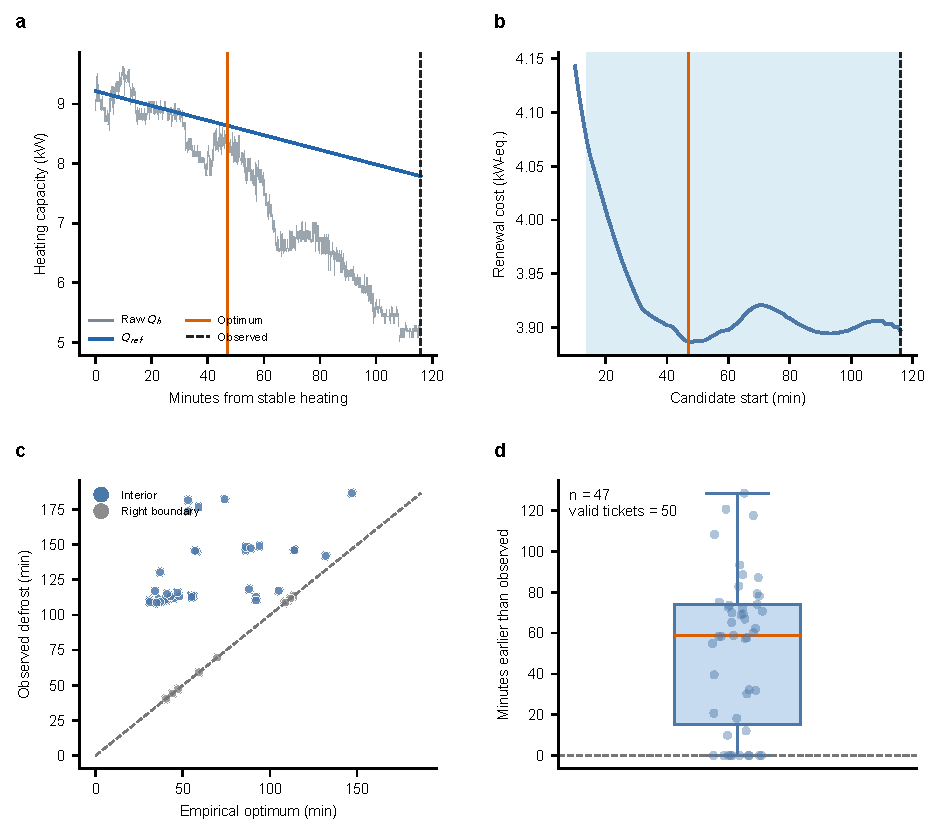
\includegraphics[width=\linewidth]{figure_1_cost.pdf}
\caption{未平滑原始数据得到固定经验门票下的逐循环离线最优点。阴影表示低遗憾候选区；竖线区分经验最小点与观察到的除霜动作。完整的59页逐循环图集见补充材料。}
\label{fig:cost}
\end{figure}

\subsection{低遗憾区显示单一最优时刻并不尖锐}
Tier~A的$t_i^*$相对实际除霜提前量中位数为58.8分钟，但其跨循环离散明显：$t_i^*$的四分位距为50.0分钟，中位数为56.0分钟。更重要的是，相对最小成本不超过1\%、2\%、5\%和10\%的时间带宽度中位数依次为33.0、52.0、95.0和102.8分钟。三个循环还包含不连续的低遗憾片段。因此，标签必须按每张图像对应时刻的pointwise regret生成，不能把两个低成本片段之间的高成本区错误填成“近最优”（图\ref{fig:labels}）。

\begin{figure}[htbp]
\centering
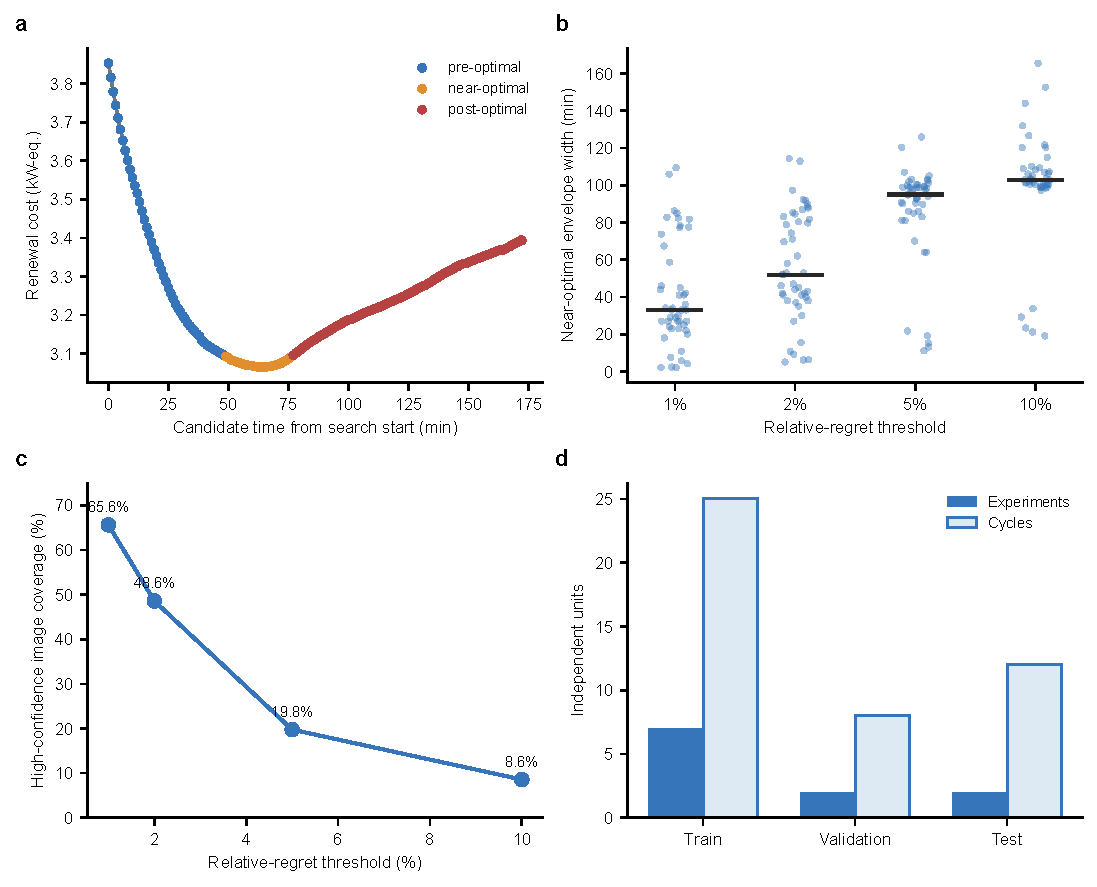
\includegraphics[width=0.92\linewidth]{figure_2_labels.pdf}
\caption{逐时刻相对遗憾把宽而可能不连续的成本谷转换为pre-optimal、near-optimal和post-optimal视觉状态。主二分类排除$\leq1\%$的低遗憾模糊区。}
\label{fig:labels}
\end{figure}

\subsection{视觉增量依赖机位，模型复杂度并非主要瓶颈}
在45个具有图像和完整成本候选域的循环中，我们以实验为单位实施leave-one-experiment-out，避免同实验帧泄露。先前锁定的RBF-SVM分析显示，全机位pooled RGB平衡准确率为0.951（0.930--0.971），但相对回顾性时间对照的配对增量区间跨零；前视机位RGB为0.965（0.942--0.987），其相对时间对照的探索性增量为0.038（0.006--0.081）（图\ref{fig:increment}）。归一化候选进度使用未来观察终点，只能作为回顾性诊断，不能直接部署在线。

\begin{figure}[htbp]
\centering
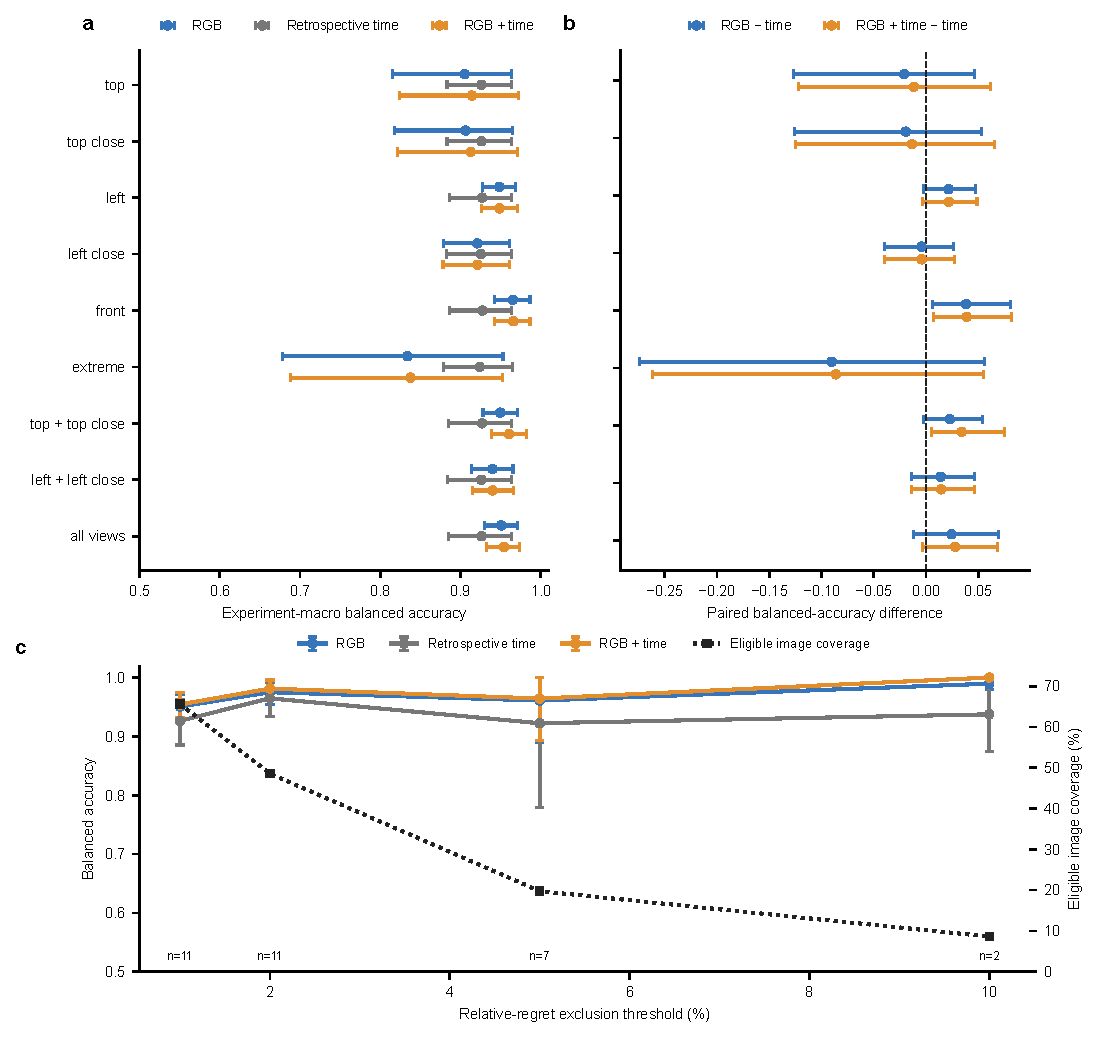
\includegraphics[width=\linewidth]{figure_3_rgb_increment.pdf}
\caption{RGB、回顾性时间及RGB+时间在未见实验中的比较。`top pair'、`left pair'和`all'表示pooled training，不是同一时刻的同步多视角融合。}
\label{fig:increment}
\end{figure}

为了区分输入信号与模型选择，我们在同一40维冻结颜色--梯度特征、同一1\%标签和同一实验折上统一比较逻辑回归、随机森林、RBF-SVM、直方图梯度提升和单隐层MLP（图\ref{fig:models}）。前视机位五种模型的平衡准确率均在0.953--0.965之间；最佳为RBF-SVM。全机位pooled的最佳结果为0.951，未超过最佳单机位。模型间差异小于机位间差异，说明当前主要瓶颈是观察视角与输入信息，而非分类器容量。

\begin{figure}[htbp]
\centering
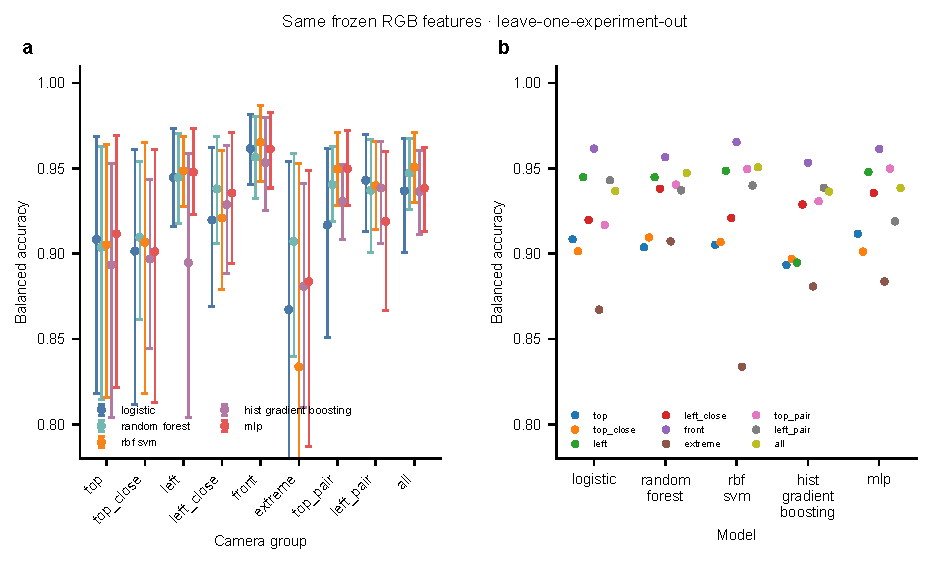
\includegraphics[width=\linewidth]{figure_5_models.pdf}
\caption{九个机位组与五种模型的统一比较。a，同一机位内比较模型；b，同一模型下比较机位。点为实验宏平均，a中的误差线为95\%实验bootstrap区间。}
\label{fig:models}
\end{figure}

实验级误差仍不可忽略（图\ref{fig:failure}）。错误主要集中在1--2\%遗憾附近，而远离最优区的错误明显减少。这说明平衡准确率需要与误分类遗憾共同报告：把远离最优点的图像判错，对控制决策的影响大于在模糊边界附近判错。

\begin{figure}[htbp]
\centering
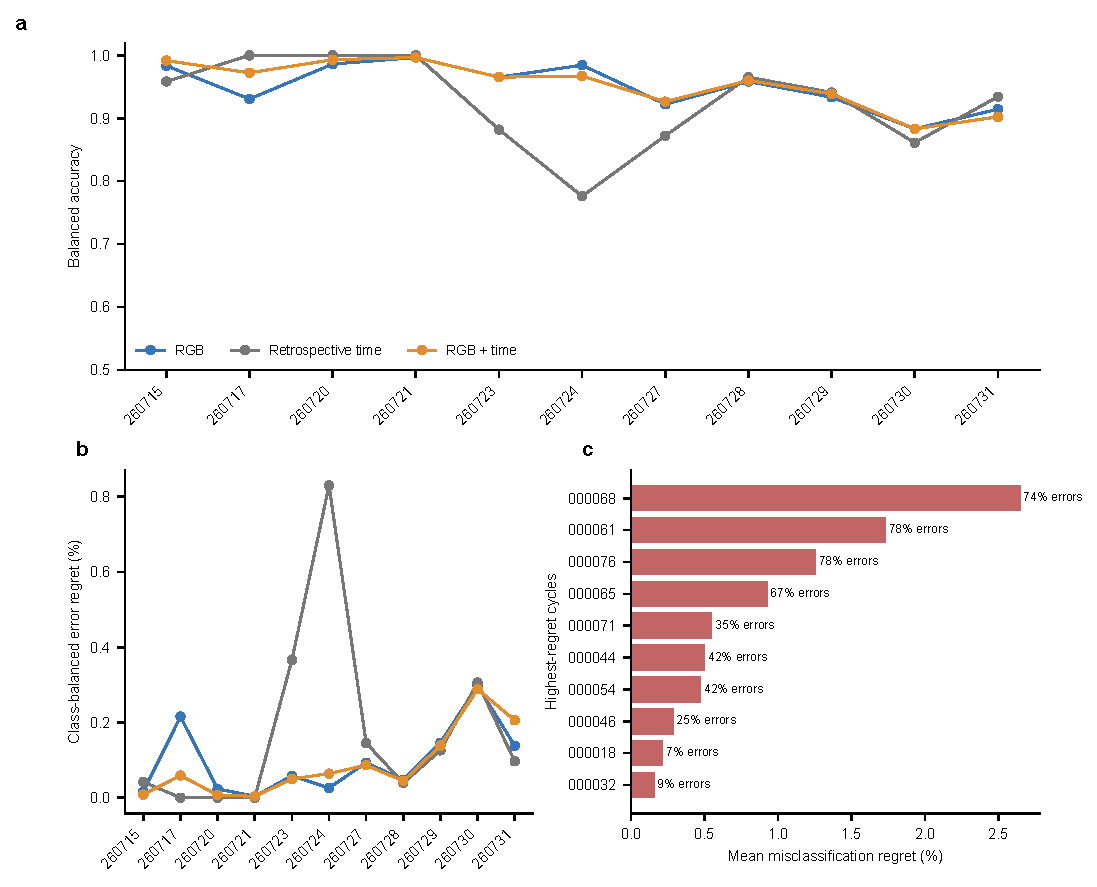
\includegraphics[width=\linewidth]{figure_4_failure.pdf}
\caption{不同实验和循环的失败审计。指标区间按独立实验重采样，而非按图像帧重采样。}
\label{fig:failure}
\end{figure}

\subsection{“最优时间分散、单帧视觉状态集中”未获支持}
为避免用监督分类准确率循环证明标签，我们在15个本地可用循环中补提pre/near/post的冻结40维特征，并比较两种逐循环质心：一是1\%低遗憾邻域，二是同一循环中、相同图片数、最接近队列中位最优分钟的固定时间图像。所有特征先在对应机位组内标准化，之后计算质心到组中心的均方根距离。分析覆盖14个可配对循环、3个独立实验。

经验最优分钟的$IQR/\mathrm{median}=0.893$，证实最优时间跨循环分散；然而九个机位组的“最优邻域减固定时间”离散度差均为正（图\ref{fig:concentration}）。全机位差值为$+0.064$（0.033--0.081），而负值才支持视觉集中。由于仅有3个本地实验，这一结果不能作为最终证伪，但足以拒绝在当前数据上宣称单帧视觉状态更集中，并触发多模态历史输入的下一阶段。

\begin{figure}[htbp]
\centering
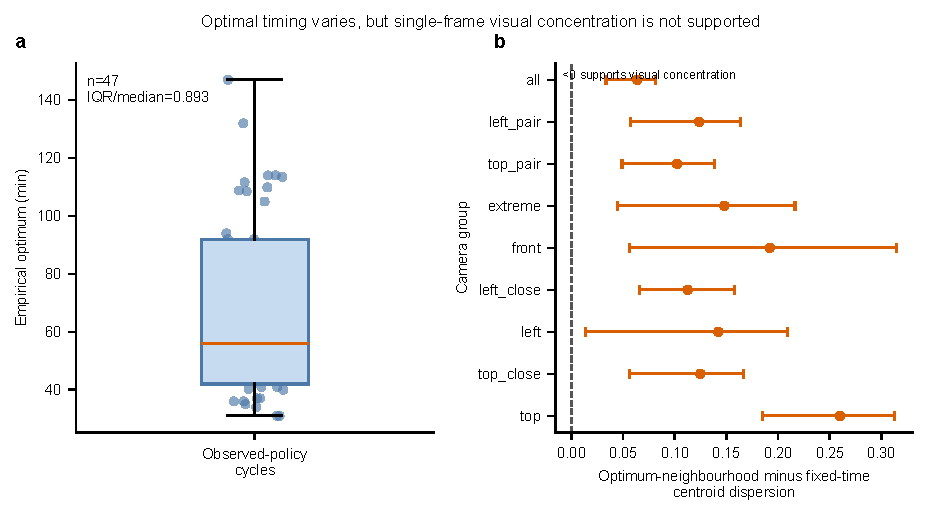
\includegraphics[width=\linewidth]{figure_6_concentration.pdf}
\caption{最优时间离散与单帧视觉集中性的直接检验。a，47个完整策略循环的经验最优分钟分布；b，最优邻域与固定时间视觉质心离散度之差。所有区间均按3个可用实验bootstrap，属于开发性证据。}
\label{fig:concentration}
\end{figure}

\section{讨论}
本研究的主要贡献不是提出又一种除霜识别网络，而是把系统成本、候选动作不确定性和视觉监督连接成同一条可审计链路。经验成本曲线使每个图像标签都能追溯到具体候选时刻及其相对遗憾；按实验隔离和时间对照则限制了帧相关性与纯时间进程造成的虚高结果。

结果同时限定了“最优除霜点”的含义。Tier~A点估计是固定观察除霜门票和离线clean reference下的最小值，并非改变动作后已观察到的反事实结果。Tier~B进一步暴露了右截尾问题：传感器记录可以扩大估计规模，但缺少实际动作与恢复锚点时，只能作为敏感性结果。宽低遗憾区说明控制器未必需要追求唯一秒级最小点；更合理的输出可能是允许动作区间或带拒绝选项的分类\citep{elyaniv2010,franc2023}。

单帧视觉分类表现较高，但“对应视觉状态更集中”的强命题没有得到当前无监督距离证据支持。可能原因包括霜形态的多路径性、光照和机位域偏移，以及相同经济损失可由不同工况组合产生。因而下一步优先级应为：在保持cycle/experiment隔离的前提下，先比较单张RGB+当前传感器，再加入传感器历史，之后才考虑多张RGB序列及同步多视角融合。只有当这些输入相对时间和传感器基线降低跨实验误分类遗憾，才有理由增加视频网络或大型视觉骨干。

cycle11因实验中途密闭环境被破坏而被目录标为invalid，已从训练、模型选择和主均值中完全隔离。其2,055条图像元数据存在，但当前没有本地特征分片；在主模型锁定后，可按单循环流式下载并作为扰动OOD压力测试，随后只删除本地临时副本而不修改云端。该结果在实际完成前不能写成已验证的泛化能力。

最后，本文没有直接室内温度、占用者暴露、PMV或PPD，因此不能把供热缺口代理写成热舒适改善；也没有随机改变除霜动作，因此不能声称已节能。决定性的后续实验应在若干低遗憾区内外主动触发除霜，直接测量电能、恢复时间、供热量和室内状态，从而检验经验成本面能否迁移到新的策略。

\section{方法}
\subsection{队列与候选域分层}
分析单位为一次稳定制热到除霜的循环。Tier~A要求catalog有效、稳定制热和实际除霜边界存在、本循环及下一循环clean anchor有效，并且原始积分覆盖率不低于95\%。Tier~B要求catalog与当前anchor有效，但允许缺失实际除霜边界；候选域止于原始传感器记录终点，并标记为right-censored。catalog invalid、候选域被长缺口截断或anchor无效的循环仅保留在审计表中。

\subsection{原始积分与经验除霜门票}
相邻有效样本间隔不超过5秒时使用梯形积分，更长缺口不桥接。除霜门票从观察到的除霜开始，止于制热量连续30秒达到下一clean anchor的90\%。门票包含实测电能和$\lambda_Q$加权供热缺口。主候选从稳定制热后10分钟开始，以1分钟网格搜索并显式包含Tier~A实际边界或Tier~B传感器终点。

\subsection{图像标签与模型评估}
候选成本遗憾按循环内时间线性插值到图像。$r\leq1\%$的图像作为near-optimal模糊区被主二分类排除；其余图像依据相对最早argmin的先后映射为0/1。九个机位组包括六个原始机位、top/top-close pooled、left/left-close pooled和全部机位pooled。五种模型共享相同40维输入和LOEO折。指标包括平衡准确率、macro-F1、AUROC和类别平衡误分类遗憾
\begin{equation}
L_r=\frac{1}{2}\sum_{y\in\{0,1\}}\frac{1}{n_y}\sum_{j:y_j=y}r_j\,\mathbf{1}(\hat y_j\neq y_j).
\end{equation}
95\%区间通过固定随机种子、5,000次实验级有放回重采样获得。

\subsection{视觉集中性检验}
集中性分析不使用分类器输出。对每个机位组，40维冻结特征先标准化；每个循环分别计算1\%低遗憾图像质心和固定中位时间附近、相同图片数的质心。每种状态的跨循环离散度定义为逐循环质心到该状态总体质心的均方根特征距离。最终比较按实验求平均的配对差，并在实验层bootstrap。

\section{数据与代码可用性}
逐循环审计、候选成本曲线、经验门票、图像标签、实验级预测以及所有主图source data均已由版本控制保存。高容量RGB原图保留在授权云端，按cycle流式物化；当前仓库中的本地临时图片不得被视为公开数据。正式投稿前仍需补充可公开仓库、版本标签、数据许可和持久标识符。

\section{结论}
本文实现了从未平滑原始运行数据、经验策略成本、低遗憾动作区到视觉分类标签的端到端演示。47个完整循环和12个右截尾循环说明经验最优点既可计算，也必须与边界类型共同解释；11实验模型比较说明机位选择比分类器复杂度更关键；3实验视觉集中性分析则阻止了一个尚不成立的强叙事。由此得到的最小下一步不是继续堆叠图像网络，而是补全cycle11扰动OOD，并检验RGB与当前/历史传感器融合能否在未见实验中降低控制遗憾。

\bibliographystyle{unsrtnat}
\bibliography{references}

\end{document}
